\documentclass{cskkuproject}
\usepackage{multirow}

% รายงานฉบับนี้แยกจาก main.tex เพื่อไม่กระทบไฟล์ตัวอย่างของเทมเพลต
\titleTH{ระบบเบลออัตโนมัติเพื่อความเป็นส่วนตัว}
\titleEN{Blur System for Privacy Protection}

\firstStudentID{663380383-1}
\firstStudentPrefixTH{นาย}
\firstStudentPrefixEN{Mr.}
\firstStudentNameTH{ณัฐภัทร วรจินดา}
\firstStudentNameEN{Nattapat Worajin}

\secondStudentID{663380606-7}
\secondStudentPrefixTH{นาย}
\secondStudentPrefixEN{Mr.}
\secondStudentNameTH{ปรเมศวร์ พุทธทองศรี}
\secondStudentNameEN{Poramet Puttongsree}

\degreeTH{วิทยาศาสตรบัณฑิต}
\degreeEN{Bachelor of Science}
\majorTH{วิทยาการคอมพิวเตอร์}
\majorEN{Computer Science}

\advisorTH{อ.ดร.พบพร ด่านวิรุทัย}
\advisorEN{Dr. Pobporn Danvirutai}

\academicYearTH{2569}
\academicYearEN{2026}
\courseCode{CP354 771}
\courseName{โครงงานคอมพิวเตอร์ 1}
\semester{1}
\projectGroup{CS 2569/CS3-9}

\keywordsTH{ความเป็นส่วนตัว, การตรวจจับใบหน้า, การเบลอภาพ, การติดตามวัตถุ, ปัญญาประดิษฐ์}
\keywordsEN{privacy protection, face detection, image redaction, object tracking, artificial intelligence}

\renewcommand{\arraystretch}{1.2}

% กล่องชั่วคราวสำหรับรูปที่ผู้จัดทำจะนำมาใส่ภายหลัง
% ไม่มีการเรียก \includegraphics จึงยังคง compile ได้เมื่อไฟล์รูปไม่พร้อม
\newcommand{\reportimageplaceholder}[2][5.5cm]{%
  \fbox{\parbox[c][#1][c]{0.86\textwidth}{\centering\textit{#2}}}%
}

% คำอธิบายเพิ่มเติมใต้ Caption ให้อยู่ใน figure เดียวกันและไม่แยกข้ามหน้า
\newcommand{\figuredescription}[2]{%
  \par\smallskip
  \begin{minipage}{0.94\textwidth}%
    \setlength{\parindent}{0pt}%
    \setlength{\leftskip}{0pt}%
    \setlength{\rightskip}{0pt}%
    \setlength{\parfillskip}{0pt plus 1fil}%
    \textbf{คำอธิบายภาพที่ \ref{#1}:} #2
  \end{minipage}%
}

% แหล่งที่มาของภาพ แยกระหว่างภาพจากภายนอกและภาพที่ผู้จัดทำสร้างขึ้นเอง
\newcommand{\figuresource}[1]{%
  \par\smallskip
  \begin{minipage}{0.94\textwidth}%
    \centering\small\textbf{ที่มา:} #1
  \end{minipage}%
}

\begin{document}

\makeprogresscover{1}

\pagenumbering{arabic}
\setcounter{page}{0}
\renewcommand{\thepage}{\ThaiAlph{\value{page}}}

\begin{abstractTH}
โครงงานนี้พัฒนาระบบเว็บสำหรับลดความเสี่ยงจากการเปิดเผยตัวตนในภาพและวิดีโอ โดยใช้ปัญญาประดิษฐ์ตรวจจับใบหน้า จัดกลุ่มใบหน้าของบุคคลเดียวกัน และปกปิดพื้นที่ที่เลือกด้วยเอฟเฟกต์ Gaussian Blur, Pixelation หรือ Black Box ผู้ใช้สามารถอัปโหลดไฟล์ภาพและวิดีโอ เลือกบุคคลที่จะปกปิดจาก Face Map ตรวจผลลัพธ์ก่อนส่งออก และกำหนดพื้นที่ปกปิดด้วยตนเองสำหรับวัตถุหรือข้อมูลอื่นที่ระบบตรวจจับไม่ได้

ในการพัฒนารอบปัจจุบัน ส่วนหน้าพัฒนาด้วย Next.js, React และ TypeScript ส่วนหลังบ้านพัฒนาด้วย FastAPI, SQLAlchemy และ SQLite โดยใช้ YOLO สำหรับตรวจจับใบหน้า InsightFace/ArcFace สำหรับสร้างเวกเตอร์ลักษณะใบหน้า OpenCV สำหรับประมวลผลเฟรม และอัลกอริทึมจับคู่กรอบแบบ IoU ร่วมกับ Hungarian Algorithm สำหรับติดตามตำแหน่งใบหน้าระหว่างเฟรม ระบบบันทึกข้อมูลวิดีโอ กรอบใบหน้า บุคคลที่ตรวจพบ การเลือกเบลอ และกรอบปกปิดที่ผู้ใช้วาดไว้เพื่อใช้สร้างตัวอย่างและไฟล์ผลลัพธ์

ผลการตรวจสอบโครงสร้างโปรแกรมพบว่าฟังก์ชันหลักตั้งแต่การอัปโหลด การตรวจจับและจัดกลุ่มใบหน้า การเลือกปกปิด การวาดกรอบด้วยตนเอง การติดตามกรอบ การแสดงตัวอย่าง และการส่งออกไฟล์ได้รับการพัฒนาแล้ว อย่างไรก็ตาม การประเมินความแม่นยำและเวลาในชุดข้อมูลมาตรฐาน รวมถึงการทดสอบแบบ end-to-end ในสภาพแวดล้อมที่ตั้งค่าแบบจำลองและ Cloudinary ครบถ้วน ยังเป็นงานที่ต้องดำเนินการต่อไป

\end{abstractTH}

\begin{abstractEN}
This project develops a web-based system that reduces the risk of identity disclosure in images and videos. It applies artificial intelligence to detect faces, group appearances of the same person, and redact selected regions using Gaussian Blur, Pixelation, or Black Box effects. Users can upload image or video files, choose identities to redact from a Face Map, inspect a preview before export, and draw manual redaction regions for objects or information that the automatic detector does not cover.

The current implementation uses Next.js, React, and TypeScript for the frontend, and FastAPI, SQLAlchemy, and SQLite for the backend. YOLO is used for face detection; InsightFace/ArcFace produces face embeddings; OpenCV processes frames; and IoU matching with the Hungarian algorithm maintains face locations across frames. The system stores video metadata, detected-face locations, grouped identities, blur selections, and manually drawn regions so that previews and final exports can be rendered consistently.

Source-structure review confirms that the major workflow---uploading media, detecting and grouping faces, choosing redaction targets, drawing and tracking manual regions, previewing, and exporting---has been implemented. Benchmarking with a standard dataset and end-to-end testing in an environment configured with the model files and Cloudinary credentials remain future work.

\end{abstractEN}

\begin{acknowledgement}
คณะผู้จัดทำขอขอบพระคุณ อ.ดร.พบพร ด่านวิรุทัย อาจารย์ที่ปรึกษาโครงงาน ที่ได้ให้คำแนะนำ ข้อเสนอแนะ และแนวทางในการพัฒนาระบบเบลออัตโนมัติเพื่อความเป็นส่วนตัวตลอดระยะเวลาการดำเนินงาน

ขอขอบพระคุณคณาจารย์และบุคลากรของวิทยาลัยการคอมพิวเตอร์ มหาวิทยาลัยขอนแก่น สำหรับความรู้และทรัพยากรที่สนับสนุนการจัดทำโครงงาน รวมทั้งเพื่อนร่วมชั้นและผู้ที่ให้ข้อคิดเห็นต่อการออกแบบระบบ

คณะผู้จัดทำจะนำข้อเสนอแนะที่ได้รับไปพัฒนาการทดสอบ ปรับปรุงคุณภาพของโค้ด และเพิ่มความครอบคลุมของการปกปิดข้อมูลส่วนบุคคลในลำดับถัดไป

\end{acknowledgement}

\tableofcontents
\clearpage
\listoffigures
\clearpage
\listoftables
\clearpage

\pagenumbering{arabic}
\setcounter{page}{1}

\chapter{บทนำ}
\section{ความเป็นมาและความสำคัญของปัญหา}

ภาพและวิดีโอถูกเผยแพร่และส่งต่อได้อย่างรวดเร็วผ่านสื่อสังคมออนไลน์ ระบบกล้องวงจรปิด และพื้นที่จัดเก็บข้อมูลบนคลาวด์ แม้สื่อเหล่านี้มีประโยชน์ต่อการสื่อสารและการวิเคราะห์ข้อมูล แต่ใบหน้าของบุคคลเป็นข้อมูลชีวมิติที่อาจเชื่อมโยงไปยังตัวบุคคลได้โดยตรง การนำสื่อไปใช้ต่อโดยไม่ปกปิดจึงอาจก่อให้เกิดความเสี่ยงด้านความเป็นส่วนตัว

รายงานความก้าวหน้าของภาคการศึกษาก่อนหน้ามุ่งเน้นการออกแบบส่วนติดต่อผู้ใช้และการคัดเลือกโมเดลเบื้องต้น ในรอบปัจจุบันได้พัฒนาระบบให้เป็นกระบวนการทำงานแบบครบลำดับมากขึ้น ตั้งแต่รับไฟล์ภาพหรือวิดีโอ ตรวจจับใบหน้า จัดกลุ่มการปรากฏของบุคคลเดียวกัน เลือกบุคคลที่จะปกปิด สร้างตัวอย่างผลลัพธ์ และส่งออกไฟล์ที่ผ่านการปกปิดแล้ว

ระบบใช้โมเดลตรวจจับแบบ YOLO ซึ่งเป็นแนวคิดการตรวจจับวัตถุแบบขั้นตอนเดียวที่ให้ความสมดุลระหว่างความเร็วและความแม่นยำ ร่วมกับเวกเตอร์ลักษณะใบหน้าจาก ArcFace เพื่อช่วยรวมใบหน้าของบุคคลเดียวกันเป็นรายการเดียวใน Face Map นอกจากการปกปิดอัตโนมัติแล้ว ยังมีเครื่องมือ Manual Control ให้ผู้ใช้วาดกรอบเหนือวัตถุที่ต้องการปกปิด เช่น ป้ายทะเบียนหรือหน้าจอ และเลือกติดตามกรอบดังกล่าวต่อเนื่องในวิดีโอได้

\section{วัตถุประสงค์}

\begin{enumerate}
    \item เพื่อพัฒนาเว็บแอปพลิเคชันสำหรับตรวจจับและปกปิดใบหน้าในไฟล์ภาพและวิดีโอ
    \item เพื่อจัดกลุ่มใบหน้าของบุคคลเดียวกันและให้ผู้ใช้กำหนดว่าจะปกปิดบุคคลใดได้อย่างชัดเจน
    \item เพื่อรองรับการปกปิดข้อมูลด้วยตนเองและการติดตามกรอบสำหรับวัตถุที่อยู่นอกขอบเขตของการตรวจจับอัตโนมัติ
    \item เพื่อให้ผู้ใช้เลือกชนิดและระดับความเข้มของเอฟเฟกต์ปกปิด ตรวจผลลัพธ์ก่อนส่งออก และดาวน์โหลดไฟล์ผลลัพธ์ได้
    \item เพื่อจัดทำแนวทางทดสอบด้านความครอบคลุมของการปกปิด ความแม่นยำ และเวลาในการประมวลผลสำหรับการประเมินในขั้นถัดไป
\end{enumerate}

\section{ขอบเขตและข้อจำกัดของระบบ}

\subsection{ขอบเขต}

ระบบรองรับไฟล์ภาพนามสกุล JPG, JPEG, PNG และ WEBP และไฟล์วิดีโอนามสกุล MP4, MOV, AVI, MKV และ WEBM โดยซอร์สโค้ดกำหนดขนาดไฟล์สูงสุดไว้ 500 MB แต่การบังคับตรวจสอบขนาดก่อนบันทึกยังเป็นส่วนที่ต้องพัฒนาเพิ่มเติม ในด้านการทำงาน ระบบตรวจจับใบหน้าในเฟรมภาพหรือวิดีโอ สร้างรายการบุคคลจากเวกเตอร์ลักษณะ (embedding) และจัดเก็บตำแหน่งที่ตรวจพบไว้ตามเฟรม ผู้ใช้สามารถเลือกปกปิดทุกคน เลือกเฉพาะบางคน หรือปกปิดทุกคนยกเว้นบุคคลที่เลือกได้

การปกปิดรองรับ Gaussian Blur, Pixelation และ Black Box พร้อมค่าความเข้มที่ปรับได้ นอกจากนี้ผู้ใช้ยังวาด ย้าย ปรับขนาด หรือลบกรอบ Manual Blur ได้ กรอบที่เปิดโหมดติดตามจะใช้ตัวติดตาม KCF หรือ CSRT ของ OpenCV ตามความพร้อมของไลบรารี เพื่อพยายามติดตามวัตถุหลังเฟรมเริ่มต้น

\subsection{ข้อจำกัดของโครงงาน}

การตรวจจับอัตโนมัติในปัจจุบันครอบคลุมใบหน้าเป็นหลัก ยังไม่มีแบบจำลองตรวจจับป้ายทะเบียนหรือข้อความส่วนบุคคลแบบอัตโนมัติ จึงต้องใช้ Manual Control กับข้อมูลประเภทดังกล่าว ความแม่นยำของการจัดกลุ่มใบหน้าขึ้นกับคุณภาพของภาพ มุมหน้า แสง การบดบังใบหน้า และค่าเกณฑ์ (threshold) ที่ใช้เปรียบเทียบเวกเตอร์ลักษณะ

การประมวลผลวิดีโอทำแบบเฟรมต่อเฟรม จึงใช้เวลาและทรัพยากรตามความยาวและความละเอียดของวิดีโอ สถานะงานเบื้องหลังถูกเก็บในหน่วยความจำของเซิร์ฟเวอร์ และการอัปโหลดผลลัพธ์ไป Cloudinary ต้องมีการกำหนดข้อมูลรับรองที่ถูกต้องก่อนใช้งานจริง

\section{ประโยชน์ที่คาดว่าจะได้รับ}

\begin{enumerate}
    \item ได้ต้นแบบเครื่องมือปกปิดใบหน้าที่ช่วยลดโอกาสเปิดเผยตัวตนก่อนเผยแพร่ภาพหรือวิดีโอ
    \item ผู้ใช้สามารถควบคุมผลการปกปิดรายบุคคลและปรับรูปแบบการปกปิดให้เหมาะกับบริบทของสื่อ
    \item ได้แนวทางผสานการตรวจจับใบหน้า การรู้จำใบหน้า การติดตามวัตถุ และการประมวลผลวิดีโอเข้ากับเว็บแอปพลิเคชัน
    \item ได้ฐานสำหรับต่อยอดการตรวจจับป้ายทะเบียน ข้อความ หรือข้อมูลส่วนบุคคลประเภทอื่น และสำหรับประเมินประสิทธิภาพเชิงปริมาณต่อไป
\end{enumerate}

\chapter{ทฤษฎีและงานวิจัยที่เกี่ยวข้อง}
\section{ทฤษฎีที่เกี่ยวข้อง}

\subsection{การปกปิดข้อมูลในภาพและวิดีโอ}

การปกปิดข้อมูลภาพ (image obfuscation) เป็นกระบวนการลดรายละเอียดของบริเวณที่อาจเปิดเผยตัวตน โดยพยายามคงบริบทส่วนอื่นของภาพหรือวิดีโอให้สามารถนำไปใช้งานต่อได้ วิธีที่ใช้ในโครงงานประกอบด้วย Gaussian Blur, Pixelation และ Black Box วิธีแรกทำให้ค่าพิกเซลในบริเวณเป้าหมายเรียบขึ้นด้วยตัวกรองแบบเกาส์ วิธีที่สองลดความละเอียดเฉพาะบริเวณแล้วขยายกลับด้วยการประมาณค่าแบบเพื่อนบ้านใกล้ที่สุด ส่วนวิธีสุดท้ายแทนที่บริเวณเป้าหมายด้วยสีทึบทั้งหมด การเลือกระดับการปกปิดต้องคำนึงถึงทั้งความเป็นส่วนตัวและประโยชน์ใช้สอยของสื่อ เพราะการปกปิดที่อ่อนเกินไปอาจยังระบุตัวบุคคลได้ ขณะที่การปกปิดมากเกินไปอาจทำลายสาระสำคัญของภาพ

ระบบใช้ OpenCV สำหรับอ่าน เขียน และปรับแต่งเฟรมภาพหรือวิดีโอ\cite{bradski2000opencv} ก่อนใช้เอฟเฟกต์ ระบบจะตรวจสอบและจำกัดพิกัดกรอบให้อยู่ภายในขนาดเฟรมเสมอ เพื่อลดความผิดพลาดจากพิกัดที่ติดลบหรือเกินขอบภาพ

\subsection{Convolutional Neural Network(CNN)}

โครงข่ายประสาทเทียมแบบคอนโวลูชัน (Convolutional Neural Network: CNN) เป็นสถาปัตยกรรมที่ออกแบบให้เรียนรู้ลักษณะเชิงพื้นที่จากภาพโดยตรง ชั้นคอนโวลูชันใช้ตัวกรองขนาดเล็กเลื่อนไปบนภาพเพื่อสกัดลักษณะ เช่น ขอบ รูปร่าง และพื้นผิว ชั้นรวมค่า (pooling) ลดมิติของแผนที่ลักษณะและช่วยให้แบบจำลองทนต่อการเลื่อนตำแหน่งเล็กน้อย ส่วนชั้นเชื่อมต่อเต็มรูปแบบหรือชั้นทำนายจะรวมลักษณะที่เรียนรู้เพื่อจำแนกประเภทหรือประมาณตำแหน่งวัตถุ CNN จึงเป็นพื้นฐานสำคัญของทั้งตัวตรวจจับใบหน้าและแบบจำลองสร้างเวกเตอร์ลักษณะใบหน้าที่ใช้ในระบบ

\subsection{การตรวจจับใบหน้าหรือวัตถุด้วย YOLO}

YOLO หรือ You Only Look Once คือการตรวจจับวัตถุแบบเรียลไทม์ มีเป้าหมายในการระบุตำแหน่งและประเภทของวัตถุในภาพ ซึ่ง YOLO จะประมวลผลภาพในขั้นตอนเดียวและทำนายกรอบล้อมวัตถุพร้อมค่าความเชื่อมั่น\cite{redmon2016yolo} จึงเหมาะกับการประมวลผลเฟรมวิดีโอที่ต้องคำนึงถึงเวลา

ความโดดเด่นของ YOLO คือสามารถตรวจจับแม้กระทั่งวัตถุที่ซ้อนทับกันโดยมีโครงสร้างที่ค่อนข้างซับซ้อนของ grid ในแต่ละชั้นที่เล็กลงเรื่อยๆในแต่ละ layers

\subsection{วิธีตรวจจับใบหน้าแบบ Haar Cascade}

Haar Cascade เป็นวิธีตรวจจับวัตถุแบบดั้งเดิมที่ประเมินความแตกต่างของความเข้มระหว่างบริเวณสว่างและมืดด้วยคุณลักษณะคล้าย Haar การคำนวณผลรวมพิกเซลสามารถเร่งได้ด้วย integral image จากนั้น AdaBoost จะคัดเลือกคุณลักษณะที่จำแนกตัวอย่างบวกและลบได้ดี และจัดตัวจำแนกเป็นลำดับขั้น (cascade) เพื่อปฏิเสธบริเวณที่ไม่ใช่ใบหน้าอย่างรวดเร็ว\cite{viola2001}

วิธีนี้ใช้ทรัพยากรน้อยและทำงานแบบเวลาจริงได้ แต่ความแม่นยำอาจลดลงเมื่อใบหน้าเอียง แสงเปลี่ยนมาก หรือมีสิ่งบดบัง จึงนำมาอธิบายเพื่อแสดงพัฒนาการของงานตรวจจับใบหน้าและใช้เป็นแนวทางเปรียบเทียบกับแบบจำลองเชิงลึกในระบบปัจจุบัน


% ==================================================
% TODO IMAGE: ใส่ภาพประกอบทฤษฎีชนิดของคุณลักษณะ Haar
% Caption: ตัวอย่างคุณลักษณะ Haar แบบขอบ แบบเส้น และแบบสี่สี่เหลี่ยม
% หมายเหตุ: ตรวจสอบแหล่งที่มาของภาพและสิทธิ์การใช้งานก่อนนำมาใส่
% ==================================================
\begin{figure}[H]
\centering
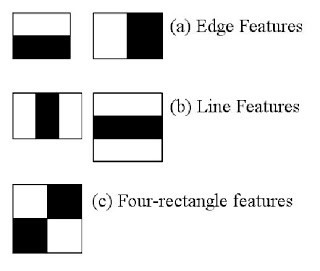
\includegraphics[width=0.8\textwidth]{images-progress/Haar feature.jpg}
\caption{ตัวอย่างคุณลักษณะ Haar แบบขอบ แบบเส้น และแบบสี่สี่เหลี่ยมที่ใช้ในตัวจำแนกแบบ Cascade}
\label{fig:haar-features}
\figuresource{OpenCV (ม.ป.ป.) \cite{opencv_haar_features}}
\figuredescription{fig:haar-features}{พื้นที่สีขาวและสีดำแทนบริเวณที่นำผลรวมค่าความเข้มของพิกเซลมาเปรียบเทียบ ภาพแสดงคุณลักษณะสามกลุ่ม ได้แก่ คุณลักษณะแบบขอบ (Edge Features) แบบเส้น (Line Features) และแบบสี่สี่เหลี่ยม (Four-rectangle Features) ซึ่งใช้ตรวจหารูปแบบความสว่างและความมืดที่สัมพันธ์กับส่วนประกอบของใบหน้า}
\end{figure}

\subsection{Support Vector Machine(SVM)}

Support Vector Machine: SVM เป็นวิธีการเรียนรู้แบบมีผู้สอนที่สร้างเส้นหรือระนาบแบ่งคลาส โดยกำหนดให้ระยะขอบระหว่างคลาสกว้างที่สุด ตัวอย่างที่อยู่ใกล้ระนาบแบ่งเรียกว่า support vectors และมีอิทธิพลต่อขอบเขตการตัดสินใจมากที่สุด สำหรับข้อมูลที่ไม่สามารถแบ่งเชิงเส้นได้ สามารถใช้ฟังก์ชันเคอร์เนลเพื่อแทนความสัมพันธ์ของข้อมูลในปริภูมิที่มีมิติสูงขึ้น

ในงานรู้จำใบหน้า SVM มักรับเวกเตอร์ลักษณะที่ผ่านการสกัดและลดมิติมาแล้วเพื่อจำแนกบุคคล อย่างไรก็ตาม ระบบปัจจุบันใช้การเปรียบเทียบเวกเตอร์ ArcFace ด้วย cosine similarity จึงกล่าวถึง SVM ในฐานะวิธีจำแนกทางเลือก ไม่ใช่ส่วนประกอบที่ใช้งานจริงในระบบ

\subsection{การรู้จำใบหน้าและการแทนลักษณะ}

การรู้จำใบหน้ามีเป้าหมายในการตรวจสอบหรือระบุอัตลักษณ์จากลักษณะของใบหน้า กระบวนการทั่วไปประกอบด้วยการปรับแนวใบหน้า การสกัดลักษณะ การสร้างตัวแทนเชิงตัวเลข และการเปรียบเทียบความคล้าย ระบบรู้จำใบหน้าต้องคำนึงถึงความเสี่ยงจากข้อมูลฝึก การรั่วไหลของตัวแทนใบหน้า และการนำผลไปใช้เกินวัตถุประสงค์\cite{sun2025}

ด้วยเหตุนี้ โครงงานจึงใช้ผลการรู้จำเพื่อจัดกลุ่มบุคคลภายในสื่อที่กำลังประมวลผลและให้ผู้ใช้ควบคุมการปกปิด โดยไม่เปิดเผยชื่อหรือข้อมูลอัตลักษณ์จริงของบุคคลที่ตรวจพบ

\subsubsection{Principal Component Analysis และ Eigenfaces}

Principal Component Analysis (PCA) ลดมิติข้อมูลโดยหาทิศทางที่มีความแปรปรวนสูง เมื่อประยุกต์กับใบหน้า ภาพแต่ละภาพถูกแปลงเป็นเวกเตอร์ $x_i$ และคำนวณใบหน้าเฉลี่ย
\begin{equation}
\psi=\frac{1}{m}\sum_{i=1}^{m}x_i.
\end{equation}
จากนั้นหาความแตกต่าง $a_i=x_i-\psi$ และสร้างเมทริกซ์ $A=[a_1,a_2,\ldots,a_m]$ เวกเตอร์ลักษณะเฉพาะที่สำคัญของเมทริกซ์ความแปรปรวนร่วมเป็นฐานของใบหน้าไอเกน (eigenfaces) ภาพใบหน้าสามารถประมาณในปริภูมิลดมิติได้เป็น
\begin{equation}
x_i-\psi \approx \sum_{j=1}^{K}w_j u_j,
\end{equation}
เมื่อ $u_j$ คือใบหน้าไอเกนและ $w_j$ คือน้ำหนักของภาพ วิธีนี้ลดภาระการคำนวณและใช้เปรียบเทียบใบหน้าได้ แต่ไวต่อแสง ท่าทาง และสิ่งบดบังมากกว่าวิธีเชิงลึกสมัยใหม่

% ==================================================
% TODO IMAGE: ใส่ภาพประกอบทฤษฎี Eigenfaces จากกระบวนการ PCA
% Caption: ตัวอย่างใบหน้าไอเกนจากกระบวนการ PCA
% แหล่งภาพที่ระบุใน Word: GeeksforGeeks, Face Recognition Using Eigenfaces
% ==================================================
\begin{figure}[H]
\centering
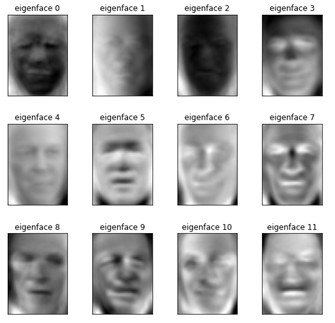
\includegraphics[width=0.8\textwidth]{images-progress/Face Recognition.jpg}
\caption{ตัวอย่างใบหน้าไอเกนจากกระบวนการ PCA}
\label{fig:pca-eigenfaces}
\figuresource{GeeksforGeeks (2021) \cite{geeksforgeeks2021eigenfaces}}
\figuredescription{fig:pca-eigenfaces}{ภาพแสดงใบหน้าไอเกนจำนวน 12 องค์ประกอบ โดยแต่ละองค์ประกอบแทนทิศทางความแปรปรวนหลักของข้อมูลใบหน้า เมื่อนำองค์ประกอบเหล่านี้มารวมกันด้วยค่าน้ำหนักที่เหมาะสมจะสามารถประมาณภาพใบหน้าในปริภูมิที่มีมิติลดลงได้}
\end{figure}

\subsubsection{Linear Discriminant Analysis และ Fisherfaces}

Linear Discriminant Analysis (LDA) เลือกทิศทางฉายข้อมูลที่เพิ่มความแตกต่างระหว่างคลาสและลดการกระจายภายในคลาส เมื่อนำมาใช้กับใบหน้า ตัวแทนที่ได้มักเรียกว่า Fisherfaces วิธีนี้ใช้ข้อมูลป้ายกำกับของบุคคลและอาจทนต่อความแปรผันภายในบุคคลได้ดีกว่า PCA ในบางกรณี อย่างไรก็ตาม ประสิทธิภาพยังขึ้นกับจำนวนและความหลากหลายของตัวอย่างฝึก

% ==================================================
% TODO IMAGE: ใส่ภาพประกอบทฤษฎี Fisherfaces จากกระบวนการ LDA
% Caption: ตัวอย่างใบหน้า Fisherfaces จากกระบวนการ LDA
% แหล่งภาพที่ระบุใน Word: BaseApp, Linear Discriminant Analysis
% ==================================================
\begin{figure}[H]
\centering
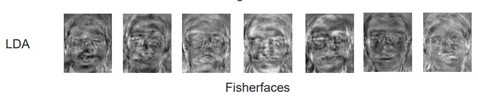
\includegraphics[width=0.8\textwidth]{images-progress/Fisherfaces.jpg}
\caption{ตัวอย่างใบหน้า Fisherfaces จากกระบวนการ LDA}
\label{fig:lda-fisherfaces}
\figuresource{Scholarpedia (ม.ป.ป.) \cite{scholarpedia_fisherfaces}}
\figuredescription{fig:lda-fisherfaces}{ภาพแสดงตัวแทน Fisherfaces ที่ได้จากการฉายข้อมูลด้วย LDA ซึ่งมุ่งเน้นลักษณะที่ช่วยเพิ่มความแตกต่างระหว่างกลุ่มบุคคลและลดความแปรปรวนของตัวอย่างภายในบุคคลเดียวกัน}
\end{figure}

\subsubsection{Elastic Bunch Graph Matching}

Elastic Bunch Graph Matching (EBGM) แทนใบหน้าเป็นกราฟของจุดสำคัญ เช่น ดวงตา จมูก และมุมปาก แต่ละจุดอธิบายด้วยผลตอบสนองของ Gabor wavelet และเชื่อมโยงกันด้วยความสัมพันธ์เชิงเรขาคณิต เมื่อเปรียบเทียบใบหน้า ระบบจะปรับกราฟให้สอดคล้องกับภาพใหม่แล้ววัดความคล้ายของลักษณะเฉพาะและตำแหน่งจุด วิธีนี้อธิบายโครงสร้างใบหน้าได้ชัดเจน แต่มีต้นทุนการกำหนดจุดและการจับคู่สูงกว่าแนวทางที่ใช้เวกเตอร์ลักษณะในระบบปัจจุบัน

% ==================================================
% TODO IMAGE: ใส่ภาพประกอบทฤษฎีการกำหนดจุดสำคัญบนใบหน้าด้วย EBGM
% Caption: การเปรียบเทียบจุดสำคัญที่กำหนดด้วยมือและตรวจจับอัตโนมัติด้วย Gabor-EBGM และ HOG-EBGM
% แหล่งภาพที่ระบุใน Word: ScienceDirect, Elastic Bunch Graph Matching
% ==================================================
\begin{figure}[H]
\centering
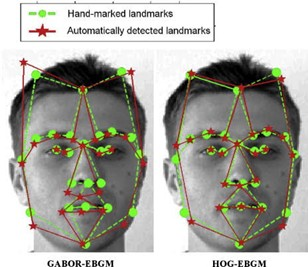
\includegraphics[width=0.8\textwidth]{images-progress/EBGM.jpg}
\caption{การเปรียบเทียบจุดสำคัญที่กำหนดด้วยมือและตรวจจับอัตโนมัติด้วย Gabor-EBGM และ HOG-EBGM}
\label{fig:ebgm-landmarks}
\figuresource{Albiol และคณะ (2008) \cite{albiol2008hogebgm}}
\figuredescription{fig:ebgm-landmarks}{วงกลมสีเขียวแสดงจุดสำคัญที่กำหนดด้วยมือ ส่วนสัญลักษณ์ดาวสีแดงแสดงจุดที่ตรวจจับโดยอัตโนมัติ ภาพด้านซ้ายเป็นผลของ Gabor-EBGM และภาพด้านขวาเป็นผลของ HOG-EBGM โดยเส้นเชื่อมระหว่างจุดแสดงโครงสร้างเชิงเรขาคณิตที่ใช้ประกอบการจับคู่ใบหน้า}
\end{figure}

\subsubsection{ArcFace และการจัดกลุ่มบุคคล}

ArcFace เป็นวิธีสร้างเวกเตอร์ลักษณะใบหน้าที่เพิ่ม angular margin ระหว่างคลาส เพื่อให้ตัวแทนของบุคคลต่างกันแยกออกจากกันได้ชัดเจนขึ้น\cite{deng2019arcface} การเปรียบเทียบเวกเตอร์สามารถใช้ cosine similarity เพื่อวัดความคล้ายระหว่างใบหน้า

ระบบปัจจุบันตัดภาพบริเวณใบหน้าพร้อมขยายขอบเขตบางส่วน แล้วสร้างเวกเตอร์ลักษณะด้วย InsightFace/ArcFace จากนั้นจึงปรับเวกเตอร์ให้มีขนาดหนึ่งและเปรียบเทียบกับกลุ่มบุคคลเดิม หากค่าความคล้ายผ่านเกณฑ์ที่กำหนด ระบบจะรวมใบหน้าเข้ากับกลุ่มเดิม มิฉะนั้นจะสร้างกลุ่มใหม่ กระบวนการนี้ทำให้ผู้ใช้เห็น Face Map เป็นรายการบุคคลแทนการเลือกกรอบใบหน้าทีละเฟรม

\subsection{การติดตามกรอบวัตถุ}

กรอบที่ตรวจพบระหว่างเฟรมถูกจับคู่ด้วยค่า Intersection over Union (IoU) และ Hungarian Algorithm หลักการดังกล่าวสอดคล้องกับการติดตามหลายวัตถุแบบออนไลน์ เช่น SORT\cite{bewley2016sort} ตัวติดตามในระบบเก็บอายุ จำนวนครั้งที่ตรวจพบ และความเร็วโดยประมาณของแต่ละกรอบ เพื่อลดการสูญหายของตำแหน่งในช่วงเวลาสั้น ๆ

สำหรับ Manual Control ระบบใช้ KCF เป็นตัวเลือกแรกและใช้ CSRT เมื่อ KCF ไม่พร้อม เพื่อให้กรอบที่ผู้ใช้วาดเคลื่อนตามวัตถุในวิดีโอ

\subsection{การตรวจจับข้อความและข้อมูลส่วนบุคคลจากข้อความ}

Optical Character Recognition (OCR) แปลงตัวอักษรในภาพเป็นข้อความดิจิทัล ส่วน Natural Language Processing (NLP) สามารถนำข้อความดังกล่าวไปจำแนกหรือระบุหน่วยข้อมูล เช่น ชื่อ หมายเลขโทรศัพท์ หรือข้อมูลส่วนบุคคลประเภทอื่น

แนวทางนี้มีประโยชน์ต่อการปกปิดข้อมูลที่ไม่ใช่ใบหน้า แต่ยังไม่ได้เชื่อมเข้ากับระบบต้นแบบปัจจุบัน จึงกำหนดไว้เป็นแนวทางพัฒนาต่อ โดยต้องประเมินทั้งความถูกต้องของ OCR และความครอบคลุมของตัวตรวจจับข้อมูลส่วนบุคคล

\subsection{สถาปัตยกรรมเว็บแอปพลิเคชัน}

ส่วนติดต่อผู้ใช้สร้างด้วย Next.js และ React ส่วน API และงานประมวลผลสร้างด้วย FastAPI ซึ่งรองรับการพัฒนา API ด้วยภาษา Python และการทำงานแบบ asynchronous\cite{fastapi} โดย Next.js ทำหน้าที่เป็นชั้น route handler ที่ส่งต่อคำขอจากเบราว์เซอร์ไปยัง FastAPI เพื่อลดการผูกส่วนหน้ากับตำแหน่งของส่วนหลังโดยตรง

ข้อมูลเมตาของวิดีโอและผลการตรวจจับจัดเก็บผ่าน SQLAlchemy ลงในฐานข้อมูล SQLite สำหรับระบบต้นแบบ ส่วนไฟล์ผลลัพธ์สามารถอัปโหลดไปยัง Cloudinary เมื่อมีการกำหนดข้อมูลรับรองที่จำเป็น

\section{งานวิจัยและงานที่เกี่ยวข้อง}

งานด้าน privacy-preserving video analytics ต้องแก้ปัญหาต่อเนื่องอย่างน้อยสามส่วน ได้แก่ การตรวจจับเป้าหมาย การติดตามเป้าหมายข้ามเฟรม และการปกปิดข้อมูลโดยยังคงประโยชน์ใช้สอยของสื่อไว้ PrivacyProber เสนอแนวทางประเมินและตรวจจับเทคนิคการเพิ่มความเป็นส่วนตัวเชิงซอฟต์ไบโอเมตริกซ์ ซึ่งสะท้อนว่าการประเมินความเป็นส่วนตัวไม่ควรพิจารณาเพียงว่ามีเอฟเฟกต์ปกปิดหรือไม่ แต่ต้องพิจารณาความสามารถในการดึงลักษณะระบุตัวตนหลังการปกปิดด้วย\cite{rot2022}

งานด้านป้ายทะเบียนแสดงให้เห็นว่าข้อมูลระบุตัวบุคคลในภาพไม่ได้จำกัดอยู่ที่ใบหน้า ทั้งงานสำรวจวิธีตรวจจับป้ายทะเบียน\cite{iiieta_anpr} ระบบจดจำป้ายทะเบียนที่ใช้ YOLOv8\cite{mdpi_anpr} และงานศึกษาการโจมตีเชิงปฏิปักษ์ต่อระบบอ่านป้ายทะเบียน\cite{vizcarra2024} ล้วนชี้ถึงความจำเป็นของการตรวจจับที่ทนต่อสภาพแวดล้อมหลากหลาย ขณะที่ชุดข้อมูลป้ายทะเบียนแบบนิรนาม\cite{anpr_dataset} เป็นตัวอย่างของการเตรียมข้อมูลที่ลดความเสี่ยงด้านความเป็นส่วนตัว

โครงงานนี้นำแนวคิดดังกล่าวมารวมเป็นเว็บแอปพลิเคชันที่ผู้ใช้ควบคุมผลการปกปิดได้เอง แตกต่างจากการเบลออัตโนมัติแบบตายตัว เพราะผู้ใช้สามารถยกเว้นบุคคลบางราย เลือกเอฟเฟกต์ และเพิ่มกรอบปกปิดให้วัตถุที่แบบจำลองยังไม่ครอบคลุม ตารางที่ \ref{tab:related-approach} สรุปความเชื่อมโยงระหว่างทฤษฎีกับส่วนที่นำไปใช้จริง

\begin{table}[H]
\centering
\caption{แนวคิดที่เกี่ยวข้องและการนำไปใช้ในระบบ}
\label{tab:related-approach}
\begin{tabular}{|p{0.28\textwidth}|p{0.30\textwidth}|p{0.27\textwidth}|}
\hline
\textbf{แนวคิด} & \textbf{บทบาท} & \textbf{การนำไปใช้} \\
\hline
YOLO & ตรวจหาตำแหน่งเป้าหมายในภาพ & ตรวจกรอบใบหน้าในแต่ละเฟรม \\
\hline
ArcFace Embedding & แยกความแตกต่างของบุคคล & จัดกลุ่มใบหน้าและสร้าง Face Map \\
\hline
IoU และ Hungarian Matching & จับคู่กรอบข้ามเฟรม & รักษากลุ่มบุคคลและตำแหน่งกรอบเมื่อวิดีโอเคลื่อนไหว \\
\hline
KCF/CSRT Tracking & ติดตามเป้าหมายที่ผู้ใช้ระบุ & ติดตามกรอบ Manual Blur ต่อจากเฟรมเริ่มต้น \\
\hline
Image Redaction & ลดการเปิดเผยข้อมูลในภาพ & Gaussian Blur, Pixelation และ Black Box \\
\hline
OCR/NLP & ตรวจข้อมูลส่วนบุคคลจากข้อความ & แนวทางพัฒนาต่อ ยังไม่รวมในระบบปัจจุบัน \\
\hline
\end{tabular}
\end{table}

\chapter{วิธีการดำเนินโครงงาน}
\section{ขั้นตอนการดำเนินงาน}

การพัฒนาใช้แนวทางวนรอบระหว่างการตรวจสอบความต้องการ ออกแบบ พัฒนา ตรวจสอบผล และปรับปรุง เริ่มจากทบทวนรายงานเดิมและโครงสร้างโปรแกรมที่มีอยู่ จากนั้นแยกฟังก์ชันที่พัฒนาแล้วออกจากฟังก์ชันที่ยังเป็นแผนงาน เพื่อให้ขอบเขตของรายงานสอดคล้องกับระบบปัจจุบัน

\begin{enumerate}
    \item วิเคราะห์ปัญหาความเป็นส่วนตัวและกำหนดการใช้งานหลัก ได้แก่ การปกปิดใบหน้า การเลือกบุคคล และการปกปิดด้วยตนเอง
    \item ออกแบบลำดับข้อมูลจากการอัปโหลดไฟล์ การสร้างเฟรมตัวอย่าง การตรวจจับและจัดกลุ่มใบหน้า จนถึงการสร้างไฟล์ผลลัพธ์
    \item พัฒนาส่วนหน้า ส่วน API บริการตรวจจับ การรู้จำ การติดตาม และการสร้างผลลัพธ์วิดีโอ
    \item ตรวจสอบเส้นทางการทำงานและโค้ดส่วนสำคัญ รวมถึงการตรวจ lint ของส่วนหน้า
    \item จัดทำรายการข้อจำกัดและแผนการทดสอบเชิงปริมาณในระยะต่อไป
\end{enumerate}

\section{สถาปัตยกรรมของระบบ}

ภาพที่ \ref{fig:architecture} แสดงสถาปัตยกรรมระดับสูงของระบบ ผู้ใช้ติดต่อกับส่วนหน้าที่พัฒนาด้วย Next.js ซึ่งส่งต่อคำขอไปยัง FastAPI บริการตรวจจับ การรู้จำ การติดตาม และการสร้างผลลัพธ์ทำงานภายในส่วนหลัง (backend) ข้อมูลเชิงโครงสร้างจัดเก็บใน SQLite ขณะที่ไฟล์ผลลัพธ์สามารถส่งต่อไปยัง Cloudinary ได้เมื่อกำหนดค่าที่จำเป็นไว้แล้ว

\begin{figure}[H]
\centering
\resizebox{0.96\textwidth}{!}{%
\begin{tikzpicture}[
    node distance=1.1cm and 1.2cm,
    box/.style={draw, rounded corners=3pt, minimum width=2.7cm, minimum height=1.0cm, align=center},
    data/.style={draw, cylinder, shape border rotate=90, aspect=0.25, minimum height=1.1cm, minimum width=1.5cm, align=center},
    line/.style={-{Latex[length=2mm]}, thick}
]
\node[box, fill=gray!12] (user) {ผู้ใช้\\Web Browser};
\node[box, fill=gray!12, right=of user] (next) {Next.js / React\\Route Handlers};
\node[box, fill=gray!12, right=of next] (api) {FastAPI\\Backend API};
\node[box, fill=gray!12, below=of api] (services) {YOLO, InsightFace,\\Tracking, Rendering};
\node[data, fill=gray!12, below left=of services] (db) {SQLite};
\node[box, fill=gray!12, below right=of services] (cloud) {Cloudinary\\(optional)};
\draw[line] (user) -- (next);
\draw[line] (next) -- (api);
\draw[line] (api) -- (services);
\draw[line] (services) -- (db);
\draw[line] (services) -- (cloud);
\end{tikzpicture}
}
\caption{สถาปัตยกรรมของระบบ Blur System}
\label{fig:architecture}
\end{figure}

\section{ลำดับการประมวลผลสื่อ}

หลังรับไฟล์ ระบบบันทึกข้อมูลเมตาและสร้างเฟรมตัวอย่าง ผู้ใช้จึงเลือกโหมดดำเนินการ จากนั้นระบบตรวจจับใบหน้า สร้างเวกเตอร์ลักษณะเพื่อจัดกลุ่มบุคคล และบันทึกตำแหน่งตามลำดับเฟรม เมื่อผู้ใช้กำหนดรายการที่จะปกปิดหรือเพิ่มกรอบ Manual Blur ระบบจะนำข้อมูลดังกล่าวไปสร้างตัวอย่างผลลัพธ์และส่งออกไฟล์โดยใช้เอฟเฟกต์ที่เลือก ดังภาพที่ \ref{fig:workflow}

\begin{figure}[H]
\centering
\begin{tikzpicture}[
    node distance=0.8cm,
    processbox/.style={draw, rounded corners=3pt, minimum width=4.3cm, minimum height=0.8cm, align=center, fill=gray!12},
    line/.style={-{Latex[length=2mm]}, thick}
]
\node[processbox] (a) {อัปโหลดภาพหรือวิดีโอ};
\node[processbox, below=of a] (b) {สร้างข้อมูลวิดีโอและเฟรมตัวอย่าง};
\node[processbox, below=of b] (c) {ตรวจจับใบหน้า จัดกลุ่มบุคคล และบันทึก Timeline};
\node[processbox, below=of c] (d) {เลือกบุคคล เพิ่ม Manual Blur และกำหนดเอฟเฟกต์};
\node[processbox, below=of d] (e) {สร้างตัวอย่างเพื่อให้ผู้ใช้ตรวจสอบ};
\node[processbox, below=of e] (f) {สร้างและส่งออกไฟล์ผลลัพธ์};
\draw[line] (a) -- (b);
\draw[line] (b) -- (c);
\draw[line] (c) -- (d);
\draw[line] (d) -- (e);
\draw[line] (e) -- (f);
\end{tikzpicture}
\caption{ลำดับการประมวลผลภาพและวิดีโอ}
\label{fig:workflow}
\end{figure}

\section{แผนภาพการทำงานของระบบ}

แผนภาพในส่วนนี้เรียงตามลำดับและบริบทจากไฟล์ Word ต้นฉบับ โดยจัดวางคำอธิบายไว้ใต้ภาพที่เกี่ยวข้องโดยตรงเพื่อให้ตรวจสอบความสัมพันธ์ระหว่างภาพกับเนื้อหาได้ชัดเจน

\subsection{Activity Diagram}

% ==================================================
% TODO IMAGE: ใส่ Activity Diagram การอัปโหลดสื่อเข้าสู่ระบบ
% Caption: Activity Diagram การอัปโหลดสื่อเข้าสู่ระบบ
% ==================================================
\begin{figure}[H]
\centering

\includegraphics[height=0.72\textheight,width=0.95\textwidth,keepaspectratio]{\detokenize{images-progress/activity diagram uploadfiles.jpg}}
\caption{Activity Diagram การอัปโหลดสื่อเข้าสู่ระบบ}
\label{fig:activity-upload}
\figuredescription{fig:activity-upload}{แสดงกิจกรรมตั้งแต่ผู้ใช้เลือกสื่อ ระบบตรวจสอบประเภทและขนาดไฟล์ บันทึกข้อมูล และสร้างภาพตัวอย่างสำหรับขั้นตอนถัดไป}
\end{figure}

% ==================================================
% TODO IMAGE: ใส่ Activity Diagram โหมด AI Auto-Blur
% Caption: Activity Diagram การปกปิดใบหน้าอัตโนมัติด้วย AI
% ==================================================
\begin{figure}[H]
\centering

\includegraphics[height=0.72\textheight,width=0.95\textwidth,keepaspectratio]{\detokenize{images-progress/activitydiagram ai auto blur.jpg}}
\caption{Activity Diagram การปกปิดใบหน้าอัตโนมัติด้วย AI}
\label{fig:activity-auto-blur}
\figuredescription{fig:activity-auto-blur}{แสดงกิจกรรมของโหมด AI Auto-Blur ตั้งแต่เริ่มกระบวนการตรวจจับใบหน้า จัดกลุ่มบุคคล ติดตามข้ามเฟรม และสร้างตัวอย่างที่ปกปิดใบหน้าทั้งหมดโดยอัตโนมัติ}
\end{figure}

% ==================================================
% TODO IMAGE: ใส่ Activity Diagram การตรวจจับและเลือกบุคคล
% Caption: Activity Diagram การตรวจจับและเลือกบุคคลที่ต้องการปกปิด
% ==================================================
\begin{figure}[H]
\centering

\includegraphics[height=0.72\textheight,width=0.95\textwidth,keepaspectratio]{\detokenize{images-progress/activity diagram detect and select.jpg}}
\caption{Activity Diagram การตรวจจับและเลือกบุคคลที่ต้องการปกปิด}
\label{fig:activity-detect-select}
\figuredescription{fig:activity-detect-select}{แสดงกิจกรรมการตรวจจับและจัดกลุ่มใบหน้าเป็นบุคคลบน Face Map การตรวจสอบ Timeline และการเลือกว่าจะปกปิดบุคคลที่เลือกหรือทุกคนยกเว้นบุคคลที่เลือก}
\end{figure}

% ==================================================
% TODO IMAGE: ใส่ Activity Diagram การควบคุมการปกปิดวิดีโอด้วยตนเอง
% Caption: Activity Diagram การควบคุมการปกปิดวิดีโอด้วยตนเอง
% ==================================================
\begin{figure}[H]
\centering

\includegraphics[height=0.72\textheight,width=0.95\textwidth,keepaspectratio]{\detokenize{images-progress/activity diagram manual control.jpg}}
\caption{Activity Diagram การควบคุมการปกปิดวิดีโอด้วยตนเอง}
\label{fig:activity-manual-control}
\figuredescription{fig:activity-manual-control}{แสดงกิจกรรมของ Manual Control สำหรับวาดและปรับขนาดกรอบ กำหนดการติดตามวัตถุ บันทึกกรอบ และตรวจตัวอย่างก่อนส่งออกวิดีโอ}
\end{figure}

% ==================================================
% TODO IMAGE: ใส่ Activity Diagram การปกปิดภาพนิ่งด้วยตนเอง
% Caption: Activity Diagram การปกปิดข้อมูลในภาพนิ่งด้วยตนเอง
% ==================================================
\begin{figure}[H]
\centering

\includegraphics[height=0.72\textheight,width=0.95\textwidth,keepaspectratio]{\detokenize{images-progress/activity diagram image manual redaction.jpg}}
\caption{Activity Diagram การปกปิดข้อมูลในภาพนิ่งด้วยตนเอง}
\label{fig:activity-image-redaction}
\figuredescription{fig:activity-image-redaction}{แสดงกิจกรรมการเพิ่มหรือลบพื้นที่ปกปิดบนภาพนิ่ง เลือกรูปแบบและระดับความเข้มของเอฟเฟกต์ แล้วประมวลผลและส่งออกภาพ}
\end{figure}

% ==================================================
% TODO IMAGE: ใส่ Activity Diagram การดูตัวอย่างและส่งออกไฟล์
% Caption: Activity Diagram การดูตัวอย่างและส่งออกไฟล์ผลลัพธ์
% ==================================================
\begin{figure}[H]
\centering

\includegraphics[height=0.72\textheight,width=0.95\textwidth,keepaspectratio]{\detokenize{images-progress/activity diagram preview and export.jpg}}
\caption{Activity Diagram การดูตัวอย่างและส่งออกไฟล์ผลลัพธ์}
\label{fig:activity-preview-export}
\figuredescription{fig:activity-preview-export}{แสดงกิจกรรมการตรวจตัวอย่างผลลัพธ์ การย้อนกลับไปปรับตั้งค่า การเรนเดอร์ไฟล์ความละเอียดเต็ม และการดาวน์โหลดหรือรับลิงก์ไฟล์จาก Cloudinary}
\end{figure}

\subsection{Use Case Diagram}

% ==================================================
% TODO IMAGE: ใส่ Use Case Diagram ภาพรวมของระบบ Blur System
% Caption: Use Case Diagram ภาพรวมการใช้งานระบบ Blur System
% ==================================================
\begin{figure}[H]
\centering

\includegraphics[height=0.70\textheight,width=0.88\textwidth,keepaspectratio]{\detokenize{images-progress/use case diagram.jpg}}
\caption{Use Case Diagram ภาพรวมการใช้งานระบบ Blur System}
\label{fig:use-case}
\figuredescription{fig:use-case}{สรุปขอบเขตการติดต่อระหว่างผู้ใช้กับความสามารถหลัก ได้แก่ การอัปโหลดสื่อ การเบลออัตโนมัติ การตรวจจับและเลือกบุคคล การควบคุมด้วยตนเอง การดูตัวอย่าง และการส่งออกผลลัพธ์}
\end{figure}

\subsection{System Sequence Diagram}

System Sequence Diagram แยกตามกรณีใช้งานเพื่อแสดงข้อความที่แลกเปลี่ยนระหว่างผู้ใช้ ส่วนหน้า ส่วนหลัง บริการประมวลผล และฐานข้อมูล

% ==================================================
% TODO IMAGE: ใส่ System Sequence Diagram การอัปโหลดสื่อ
% Caption: System Sequence Diagram การอัปโหลดสื่อเข้าสู่ระบบ
% ==================================================
\begin{figure}[H]
\centering

\includegraphics[height=0.72\textheight,width=0.95\textwidth,keepaspectratio]{\detokenize{images-progress/System Sequence Diagram — การอัปโหลดไฟล์สื่อ.jpg}}
\caption{System Sequence Diagram การอัปโหลดสื่อเข้าสู่ระบบ}
\label{fig:ssd-upload}
\figuredescription{fig:ssd-upload}{แสดงลำดับการตรวจสอบไฟล์ ส่งคำขออัปโหลด บันทึกข้อมูลสื่อในฐานข้อมูล สร้างภาพตัวอย่าง และส่งข้อมูลกลับไปยังส่วนหน้า}
\end{figure}

% ==================================================
% TODO IMAGE: ใส่ System Sequence Diagram โหมด AI Auto-Blur
% Caption: System Sequence Diagram การปกปิดใบหน้าอัตโนมัติด้วย AI
% ==================================================
\begin{figure}[H]
\centering

\includegraphics[height=0.72\textheight,width=0.95\textwidth,keepaspectratio]{\detokenize{images-progress/System Sequence Diagram — การเบลออัตโนมัติ.jpg}}
\caption{System Sequence Diagram การปกปิดใบหน้าอัตโนมัติด้วย AI}
\label{fig:ssd-auto-blur}
\figuredescription{fig:ssd-auto-blur}{แสดงลำดับการเริ่มงาน AI Auto-Blur การตรวจจับและสร้าง Face Embedding การจัดกลุ่มและติดตามบุคคล ตลอดจนการรายงานความคืบหน้าและสร้างตัวอย่างผลลัพธ์}
\end{figure}

% ==================================================
% TODO IMAGE: ใส่ System Sequence Diagram การตรวจจับใบหน้า
% Caption: System Sequence Diagram การตรวจจับและจัดกลุ่มใบหน้า
% ==================================================
\begin{figure}[H]
\centering

\includegraphics[height=0.72\textheight,width=0.95\textwidth,keepaspectratio]{\detokenize{images-progress/System Sequence Diagram — ตรวจจับใบหน้า.jpg}}
\caption{System Sequence Diagram การตรวจจับและจัดกลุ่มใบหน้า}
\label{fig:ssd-face-detection}
\figuredescription{fig:ssd-face-detection}{แสดงลำดับการเริ่ม Detection Pipeline การตรวจจับและจัดกลุ่มใบหน้า การบันทึกผล และการเรียกดูสถานะของงานแบบเบื้องหลัง}
\end{figure}

% ==================================================
% TODO IMAGE: ใส่ System Sequence Diagram การเลือกบุคคลและปกปิดแบบรายบุคคล
% Caption: System Sequence Diagram การเลือกบุคคลและการปกปิดแบบรายบุคคล
% ==================================================
\begin{figure}[H]
\centering

\includegraphics[height=0.72\textheight,width=0.95\textwidth,keepaspectratio]{\detokenize{images-progress/System Sequence Diagram — การเลือกบุคคลและเบลอ.jpg}}
\caption{System Sequence Diagram การเลือกบุคคลและการปกปิดแบบรายบุคคล}
\label{fig:ssd-selective-blur}
\figuredescription{fig:ssd-selective-blur}{แสดงลำดับการโหลด Face Map การเลือกบุคคลและรูปแบบการปกปิด การบันทึกค่า \texttt{should\_blur} และการสร้างตัวอย่างตามตัวเลือกของผู้ใช้}
\end{figure}

% ==================================================
% TODO IMAGE: ใส่ System Sequence Diagram การควบคุมการปกปิดด้วยตนเอง
% Caption: System Sequence Diagram การควบคุมการปกปิดวิดีโอด้วยตนเอง
% ==================================================
\begin{figure}[H]
\centering

\includegraphics[height=0.72\textheight,width=0.95\textwidth,keepaspectratio]{\detokenize{images-progress/System Sequence Diagram — Manual Control.jpg}}
\caption{System Sequence Diagram การควบคุมการปกปิดวิดีโอด้วยตนเอง}
\label{fig:ssd-manual-control}
\figuredescription{fig:ssd-manual-control}{แสดงลำดับการโหลดเฟรม วาดและบันทึกกรอบ Manual Blur การสร้างตัวติดตาม KCF/CSRT และการสร้างตัวอย่างผลลัพธ์}
\end{figure}

% ==================================================
% TODO IMAGE: ใส่ System Sequence Diagram การปกปิดภาพนิ่งด้วยตนเอง
% Caption: System Sequence Diagram การปกปิดข้อมูลในภาพนิ่งด้วยตนเอง
% ==================================================
\begin{figure}[H]
\centering

\includegraphics[height=0.72\textheight,width=0.95\textwidth,keepaspectratio]{\detokenize{images-progress/System Sequence Diagram — การเบลอรูปภาพด้วยตนเอง.jpg}}
\caption{System Sequence Diagram การปกปิดข้อมูลในภาพนิ่งด้วยตนเอง}
\label{fig:ssd-image-redaction}
\figuredescription{fig:ssd-image-redaction}{แสดงลำดับการเพิ่มหรือลบ Redaction Zone บนภาพนิ่ง การตั้งค่าเอฟเฟกต์และความเข้ม และการส่งคำขอสร้างภาพตัวอย่าง}
\end{figure}

% ==================================================
% TODO IMAGE: ใส่ System Sequence Diagram การดูตัวอย่างและส่งออกไฟล์
% Caption: System Sequence Diagram การดูตัวอย่างและส่งออกไฟล์ผลลัพธ์
% ==================================================
\begin{figure}[H]
\centering

\includegraphics[height=0.72\textheight,width=0.95\textwidth,keepaspectratio]{\detokenize{images-progress/System Sequence Diagram — การดูตัวอย่างและส่งออกไฟล์ (Preview & Export).jpg}}
\caption{System Sequence Diagram การดูตัวอย่างและส่งออกไฟล์ผลลัพธ์}
\label{fig:ssd-preview-export}
\figuredescription{fig:ssd-preview-export}{แสดงลำดับการเปิดตัวอย่าง การยืนยันส่งออก การเรนเดอร์ไฟล์ การรวมเสียงวิดีโอ การอัปโหลด Cloudinary และการส่งคืนลิงก์ดาวน์โหลด}
\end{figure}

\section{เครื่องมือที่ใช้ในการดำเนินงาน}

\begin{table}[H]
\centering
\caption{ซอฟต์แวร์และไลบรารีหลักที่ใช้ในโครงงาน}
\label{tab:tools}
\begin{tabular}{|p{0.31\textwidth}|p{0.54\textwidth}|}
\hline
\textbf{เครื่องมือ} & \textbf{การใช้งาน} \\
\hline
Next.js 16, React 19, TypeScript & สร้างส่วนติดต่อผู้ใช้และ route handler สำหรับเชื่อมต่อส่วนหลัง \\
\hline
FastAPI, Uvicorn & สร้าง REST API และรันงานตรวจจับแบบเบื้องหลัง \\
\hline
Ultralytics YOLO & ตรวจจับใบหน้า โดยมีแบบจำลองทั่วไปเป็นทางเลือกสำรอง \\
\hline
InsightFace และ ONNX Runtime & สร้างเวกเตอร์ลักษณะใบหน้าสำหรับจัดกลุ่มบุคคล \\
\hline
OpenCV, NumPy, SciPy & อ่านและเขียนสื่อ ปรับภาพ ใช้ tracker และจับคู่กรอบด้วย Hungarian algorithm \\
\hline
SQLAlchemy และ SQLite & จัดเก็บข้อมูลวิดีโอ ผลตรวจจับ กลุ่มบุคคล การเลือกปกปิด และกรอบที่กำหนดด้วยตนเอง \\
\hline
Cloudinary & จัดเก็บผลลัพธ์บนคลาวด์เมื่อกำหนดข้อมูลรับรองไว้ \\
\hline
\end{tabular}
\end{table}

\section{แผนการทดสอบและเกณฑ์การประเมิน}

การทดสอบระยะถัดไปแบ่งเป็นสามส่วน ได้แก่ (1) การทดสอบฟังก์ชันแบบ end-to-end ตั้งแต่การอัปโหลดจนถึงการส่งออกไฟล์ (2) การทดสอบความแม่นยำของการตรวจจับและความถูกต้องของการจัดกลุ่มบุคคลด้วยชุดข้อมูลที่กำหนด และ (3) การวัดเวลาเฉลี่ยต่อเฟรม เวลาสร้างผลลัพธ์ทั้งไฟล์ และความครอบคลุมของพื้นที่ปกปิด เกณฑ์เชิงคุณภาพจะตรวจสอบว่าใบหน้าที่ควรปกปิดไม่หลุดจากกรอบ และผู้ใช้สามารถแก้ไขกรณีตรวจจับผิดพลาดได้ผ่าน Manual Control

\chapter{การวิเคราะห์ ออกแบบและพัฒนาระบบ}
\section{การวิเคราะห์ระบบ}

ผู้ใช้มีเป้าหมายหลักคือการเตรียมสื่อสำหรับเผยแพร่โดยลดการเปิดเผยตัวตนของบุคคล ระบบจึงออกแบบให้เริ่มจากการอัปโหลดไฟล์ แสดงผลการตรวจจับในรูปของรายการบุคคลที่จัดกลุ่มแล้ว เปิดโอกาสให้ผู้ใช้ตัดสินใจว่าจะปกปิดหรือยกเว้นบุคคลใด และแก้ไขบริเวณที่ AI ยังตรวจจับไม่ครอบคลุมก่อนส่งออกไฟล์ ตารางที่ \ref{tab:functional-requirements} แสดงความต้องการเชิงฟังก์ชันของระบบปัจจุบัน

\begin{table}[H]
\centering
\caption{ความต้องการเชิงฟังก์ชันของระบบ}
\label{tab:functional-requirements}
\begin{tabular}{|p{0.13\textwidth}|p{0.42\textwidth}|p{0.30\textwidth}|}
\hline
\textbf{รหัส} & \textbf{ความต้องการ} & \textbf{สถานะในระบบ} \\
\hline
FR-01 & ผู้ใช้อัปโหลดภาพหรือวิดีโอที่รองรับได้ & พัฒนาแล้ว \\
\hline
FR-02 & ระบบสร้างข้อมูลเมตาและเฟรมตัวอย่างของสื่อที่อัปโหลด & พัฒนาแล้ว \\
\hline
FR-03 & ระบบตรวจจับใบหน้าและบันทึกตำแหน่งตามเฟรม & พัฒนาแล้ว \\
\hline
FR-04 & ระบบรวมใบหน้าที่คาดว่าเป็นบุคคลเดียวกันเป็นกลุ่มบุคคล & พัฒนาแล้ว \\
\hline
FR-05 & ผู้ใช้เลือกเบลอทุกคน เฉพาะคน หรือทุกคนยกเว้นคนที่เลือกได้ & พัฒนาแล้ว \\
\hline
FR-06 & ผู้ใช้กำหนด Gaussian Blur, Pixelation หรือ Black Box และปรับความเข้มได้ & พัฒนาแล้ว \\
\hline
FR-07 & ผู้ใช้วาด ย้าย ปรับขนาด ลบ และเลือกติดตามกรอบ Manual Blur ได้ & พัฒนาแล้ว \\
\hline
FR-08 & ระบบสร้างตัวอย่างและส่งออกภาพหรือวิดีโอที่ปกปิดข้อมูลแล้วได้ & พัฒนาแล้ว \\
\hline
FR-09 & ระบบส่งไฟล์ผลลัพธ์ไปยัง Cloudinary ได้เมื่อมีข้อมูลรับรอง & พัฒนาแล้วในลักษณะตัวเลือกเสริม \\
\hline
\end{tabular}
\end{table}

ความต้องการที่ไม่ใช่เชิงฟังก์ชัน ได้แก่ การป้องกันพิกัดกรอบไม่ให้เกินขนาดเฟรม การรองรับงานเบื้องหลังระหว่างตรวจจับวิดีโอ การแสดงข้อความแจ้งสถานะการทำงาน และการคงผลการเลือกปกปิดไว้ในฐานข้อมูล อย่างไรก็ตาม ซอร์สโค้ดปัจจุบันยังต้องปรับปรุงความปลอดภัยสำหรับการใช้งานจริง เช่น การกำหนด CORS ให้จำกัดโดเมน การบังคับตรวจสอบขนาดไฟล์ที่อัปโหลด และการจัดเก็บสถานะงานให้ทนทานต่อการรีสตาร์ตเซิร์ฟเวอร์

\section{การออกแบบข้อมูลและส่วนประกอบ}

ฐานข้อมูลของระบบแบ่งข้อมูลเป็นสามกลุ่ม ได้แก่ ข้อมูลสื่อ ผลการวิเคราะห์ใบหน้า และการตั้งค่าปกปิด ตารางที่ \ref{tab:data-model} สรุป entity สำคัญที่กำหนดด้วย SQLAlchemy

\begin{table}[H]
\centering
\caption{โครงสร้างข้อมูลหลักของระบบ}
\label{tab:data-model}
\begin{tabular}{|p{0.26\textwidth}|p{0.28\textwidth}|p{0.31\textwidth}|}
\hline
\textbf{ตาราง} & \textbf{ข้อมูลสำคัญ} & \textbf{บทบาท} \\
\hline
videos & ชื่อไฟล์, ขนาดเฟรม, FPS, จำนวนเฟรม, สถานะ & เก็บข้อมูลต้นทางของภาพหรือวิดีโอ \\
\hline
preview\_frames & หมายเลขเฟรม เวลา และที่อยู่ของภาพขนาดย่อ & ใช้เลือกและแสดงตัวอย่างเฟรม \\
\hline
detected\_faces & พิกัดกรอบ ค่าความเชื่อมั่น กลุ่มบุคคล และหมายเลขเฟรม & เก็บผลตรวจจับที่ใช้สร้างผลลัพธ์ \\
\hline
identities & ป้ายกำกับ ภาพขนาดย่อ เวกเตอร์ลักษณะเฉลี่ย และจำนวนการปรากฏ & แทนบุคคลแต่ละรายบน Face Map \\
\hline
blur\_selections & รหัสวิดีโอ รหัสกลุ่มบุคคล และสถานะการปกปิด & เก็บการตัดสินใจว่าจะปกปิดบุคคลใด \\
\hline
timeline\_entries & รหัสกลุ่มบุคคล หมายเลขเฟรม และเวลา & แสดงช่วงเวลาที่บุคคลปรากฏ \\
\hline
manual\_blur\_boxes & พิกัด ขนาด เฟรมเริ่มต้น และสถานะการติดตาม & เก็บพื้นที่ปกปิดที่ผู้ใช้กำหนดเอง \\
\hline
\end{tabular}
\end{table}

ส่วนหลัง (backend) แยกความรับผิดชอบเป็นบริการตรวจจับใบหน้า บริการรู้จำใบหน้า บริการติดตามวัตถุ และบริการสร้างผลลัพธ์ การแยกส่วนดังกล่าวช่วยให้เปลี่ยนแบบจำลองหรือปรับวิธีปกปิดได้โดยไม่กระทบ API หลัก ส่วนหน้า (frontend) แบ่งเป็นคอมโพเนนต์สำหรับอัปโหลดสื่อ เลือกบุคคล แสดง Timeline ควบคุมการปกปิดด้วยตนเอง และส่งออกผลลัพธ์

\section{การออกแบบส่วนติดต่อผู้ใช้}

ส่วนติดต่อผู้ใช้จัดลำดับการทำงานให้เริ่มจากการอัปโหลดสื่อ เลือกเครื่องมือ ตรวจสอบผลการตรวจจับ แก้ไขพื้นที่ปกปิด และยืนยันผลก่อนส่งออก ภาพ Demo ในส่วนนี้เรียงตามขั้นตอนการใช้งาน และวางคำอธิบายไว้ใต้ภาพที่เกี่ยวข้องโดยตรง

% ==================================================
% TODO IMAGE: ใส่ภาพ Demo หน้าจอหลักและส่วนอัปโหลดไฟล์
% Caption: หน้าจอหลักและส่วนอัปโหลดไฟล์
% ==================================================
\begin{figure}[H]
\centering

\includegraphics[width=0.94\textwidth]{\detokenize{images-progress/ภาพ demo หน้าแรก (Home).jpg}}
\caption{หน้าจอหลักและส่วนอัปโหลดไฟล์}
\label{fig:demo-home}
\figuredescription{fig:demo-home}{เป็นหน้าจอเริ่มต้นสำหรับเลือกหรือลากไฟล์ภาพและวิดีโอเข้าสู่พื้นที่อัปโหลดของระบบ}
\end{figure}

% ==================================================
% TODO IMAGE: ใส่ภาพ Demo หน้าจอเลือกเครื่องมือและตั้งค่าการประมวลผล
% Caption: หน้าจอเลือกเครื่องมือและตั้งค่าการประมวลผล
% ==================================================
\begin{figure}[H]
\centering

\includegraphics[width=0.94\textwidth]{\detokenize{images-progress/ภาพ demo หน้าการตั้งค่าการประมวลผล(Tools).jpg}}
\caption{หน้าจอเลือกเครื่องมือและตั้งค่าการประมวลผล}
\label{fig:demo-tools}
\figuredescription{fig:demo-tools}{แสดงหน้าจอเลือก AI Auto-Blur, Detect \& Select หรือ Manual Control พร้อมกำหนดรูปแบบและระดับความเข้มของการปกปิด}
\end{figure}

% ==================================================
% TODO IMAGE: ใส่ภาพ Demo หน้าจอการตรวจจับและเลือกบุคคล
% Caption: หน้าจอการตรวจจับและเลือกบุคคลที่ต้องการปกปิด
% ==================================================
\begin{figure}[H]
\centering

\includegraphics[width=0.94\textwidth]{\detokenize{images-progress/ภาพ demo หน้าเมนู Detect&Select .jpg}}
\caption{หน้าจอการตรวจจับและเลือกบุคคลที่ต้องการปกปิด}
\label{fig:demo-detect-select}
\figuredescription{fig:demo-detect-select}{แสดงผลการตรวจจับเป็น Face Map เพื่อให้ผู้ใช้ตรวจสอบบุคคลที่พบ เลือกบุคคลที่ต้องการปกปิด และกำหนดรูปแบบการปกปิด}
\end{figure}

% ==================================================
% TODO IMAGE: ใส่ภาพ Demo หน้าจอรายการคีย์เฟรมและ Timeline
% Caption: หน้าจอรายการคีย์เฟรมและช่วงเวลาที่ตรวจพบบุคคล
% ==================================================
\begin{figure}[H]
\centering

\includegraphics[width=0.94\textwidth]{\detokenize{images-progress/ภาพ demo หน้าจอแสดงจำนวน Keyframes.jpg}}
\caption{หน้าจอรายการคีย์เฟรมและช่วงเวลาที่ตรวจพบบุคคล}
\label{fig:demo-timeline}
\figuredescription{fig:demo-timeline}{แสดงรายการคีย์เฟรม หมายเลขเฟรม และเวลาที่ตรวจพบบุคคล เพื่อให้ผู้ใช้เลือกตรวจสอบช่วงสำคัญของวิดีโอได้สะดวก}
\end{figure}

% ==================================================
% TODO IMAGE: ใส่ภาพ Demo หน้าจอ Manual Control
% Caption: หน้าจอควบคุมและกำหนดพื้นที่ปกปิดด้วยตนเอง
% ==================================================
\begin{figure}[H]
\centering

\includegraphics[width=0.94\textwidth]{\detokenize{images-progress/ภาพ demo เมนู Manual Control.jpg}}
\caption{หน้าจอควบคุมและกำหนดพื้นที่ปกปิดด้วยตนเอง}
\label{fig:demo-manual-control}
\figuredescription{fig:demo-manual-control}{แสดงหน้าจอ Manual Control สำหรับวาดกรอบครอบบริเวณที่ต้องการปกปิด ปรับขนาดกรอบ และกำหนดให้กรอบติดตามวัตถุในวิดีโอ}
\end{figure}

% ==================================================
% TODO IMAGE: ใส่ภาพ Demo หน้าจอโหมด AI Auto-Blur
% Caption: หน้าจอการทำงานของโหมด AI Auto-Blur
% หมายเหตุ: ไฟล์ "ภาพ demo AI-Auto Blur.jpg" ซ้ำกับภาพ Manual Control
% จึงเว้นตำแหน่งไว้เพื่อป้องกันภาพและคำอธิบายไม่ตรงกัน
% ==================================================
\begin{figure}[H]
\centering
\reportimageplaceholder{[เว้นพื้นที่สำหรับภาพ Demo โหมด AI Auto-Blur]}
\caption{หน้าจอการทำงานของโหมด AI Auto-Blur}
\label{fig:demo-auto-blur}
\figuredescription{fig:demo-auto-blur}{ตำแหน่งนี้ใช้แสดงหน้าจอการทำงานของโหมด AI Auto-Blur ซึ่งตรวจจับและปกปิดใบหน้าโดยอัตโนมัติ เพื่อลดการกำหนดพื้นที่ทีละตำแหน่ง}
\end{figure}

% ==================================================
% TODO IMAGE: ใส่ภาพ Demo หน้าจอตรวจสอบผลลัพธ์ก่อนส่งออก
% Caption: หน้าจอตรวจสอบผลลัพธ์หลังประมวลผลก่อนส่งออกไฟล์
% ==================================================
\begin{figure}[H]
\centering

\includegraphics[width=0.94\textwidth]{\detokenize{images-progress/ภาพ หน้า Preview Result.jpg}}
\caption{หน้าจอตรวจสอบผลลัพธ์หลังประมวลผลก่อนส่งออกไฟล์}
\label{fig:demo-preview}
\figuredescription{fig:demo-preview}{เป็นหน้าจอตรวจสอบผลหลังประมวลผล ผู้ใช้สามารถเล่นวิดีโอตัวอย่างเพื่อยืนยันว่าพื้นที่เป้าหมายถูกปกปิดครบถ้วนก่อนส่งออกไฟล์}
\end{figure}

\section{การพัฒนาและการปรับปรุงจากภาคการศึกษาก่อนหน้า}

ตารางที่ \ref{tab:progress-update} เปรียบเทียบสิ่งที่รายงานเดิมระบุว่าอยู่ระหว่างพัฒนากับสภาพของซอร์สโค้ดปัจจุบัน

\begin{table}[H]
\centering
\caption{ความก้าวหน้าของระบบในรอบปัจจุบัน}
\label{tab:progress-update}
\begin{tabular}{|p{0.29\textwidth}|p{0.25\textwidth}|p{0.31\textwidth}|}
\hline
\textbf{หัวข้อ} & \textbf{สถานะในรายงานเดิม} & \textbf{สถานะปัจจุบัน} \\
\hline
ส่วนติดต่อผู้ใช้ & ออกแบบ UI/UX และทดสอบเชื่อม API & มีกระบวนการอัปโหลด Tools, Face Map, Manual Control, Preview และ Export \\
\hline
Selective Blur & พัฒนาเบื้องต้น & จัดกลุ่มบุคคลจากเวกเตอร์ลักษณะ บันทึกตัวเลือกการปกปิด และเลือกปกปิดหรือยกเว้นรายบุคคลได้ \\
\hline
การประมวลผลวิดีโอ & อยู่ระหว่างพัฒนา & มีกระบวนการตรวจจับแบบเบื้องหลัง การบันทึกตำแหน่งตามเฟรม และบริการสร้างไฟล์ผลลัพธ์ \\
\hline
Manual Override & ออกแบบหน้าจอไว้ & วาด ย้าย ปรับขนาด ลบ และบันทึกกรอบปกปิด พร้อมตัวเลือกติดตามวัตถุ \\
\hline
รูปแบบการปกปิด & กำหนดแนวทางไว้ & ใช้ Gaussian Blur, Pixelation และ Black Box พร้อมปรับระดับความเข้ม \\
\hline
Preview และ Export & ระบุเป็นหน้าผลลัพธ์ & สร้างตัวอย่างก่อนส่งออกและส่งคืน URL สำหรับดาวน์โหลดหรือเปิดผ่าน Cloudinary \\
\hline
การประเมินเชิงปริมาณ & อยู่ระหว่างพัฒนา & ยังต้องเก็บผลการประเมินประสิทธิภาพและความแม่นยำด้วยชุดทดสอบมาตรฐาน \\
\hline
\end{tabular}
\end{table}

\subsection{การตรวจจับและสร้าง Face Map}

เมื่อเริ่มกระบวนการตรวจจับ ระบบอ่านวิดีโอทีละเฟรมและเรียกบริการตรวจจับใบหน้า จากนั้นตัดภาพใบหน้าพร้อมขยายขอบเขตบางส่วนเพื่อสร้างเวกเตอร์ลักษณะ ระบบเปรียบเทียบเวกเตอร์ดังกล่าวกับค่าเฉลี่ยของกลุ่มบุคคลที่พบก่อนหน้า หากค่าความคล้ายสูงกว่าค่าเกณฑ์ ระบบจะรวมใบหน้าเข้ากับกลุ่มเดิม มิฉะนั้นจะสร้างกลุ่มบุคคลใหม่ เมื่อกระบวนการเสร็จสิ้น ระบบจะสร้างรายการ Face Map ค่าความเชื่อมั่นเฉลี่ย และ Timeline ของการปรากฏ

\subsection{การปกปิดแบบเลือกได้และการสร้างผลลัพธ์}

กลุ่มบุคคลที่สร้างขึ้นจะมีสถานะเริ่มต้นเป็นการปกปิด ระบบนำสถานะนี้ไปรวมกับตำแหน่งใบหน้าในทุกเฟรมเมื่อสร้างตัวอย่างหรือส่งออกไฟล์ หากผู้ใช้ต้องการให้ใบหน้าบางรายยังคงมองเห็น สามารถปิดสถานะการปกปิดของบุคคลนั้นได้ บริการสร้างผลลัพธ์จะตรวจสอบขอบเขตพื้นที่ก่อนใช้เอฟเฟกต์ที่ผู้ใช้เลือก และกำหนดขนาด kernel ที่เหมาะสมสำหรับ Gaussian Blur

\subsection{การปกปิดด้วยตนเองและการติดตาม}

Manual Control แสดงภาพตัวอย่างให้ผู้ใช้ลากกรอบเหนือวัตถุที่ต้องการปกปิด ตำแหน่งบนหน้าจอจะถูกแปลงกลับเป็นพิกัดจริงของภาพก่อนบันทึก สำหรับวิดีโอ ระบบจะเริ่มตัวติดตามที่เฟรมเริ่มต้นของกรอบ และนำกรอบที่ติดตามได้ไปใช้ปกปิดเฟรมถัดไป หากตัวติดตามไม่พร้อมใช้งาน ระบบจะใช้กรอบแบบคงที่เป็นทางเลือกสำรอง

\section{การตรวจสอบระบบในรอบจัดทำรายงาน}

ผลการตรวจสอบในตารางที่ \ref{tab:inspection-result} เป็นการตรวจเส้นทางการทำงานและซอร์สโค้ดปัจจุบัน ไม่ใช่ผลการประเมินประสิทธิภาพของแบบจำลองหรือผลการทดสอบกับผู้ใช้จริง จึงแยกสถานะ ``พัฒนาแล้ว'' ออกจาก ``ต้องดำเนินการต่อ'' อย่างชัดเจน

\begin{table}[H]
\centering
\caption{ผลการตรวจสอบระบบในรอบจัดทำรายงาน}
\label{tab:inspection-result}
\begin{tabular}{|p{0.13\textwidth}|p{0.38\textwidth}|p{0.34\textwidth}|}
\hline
\textbf{รายการ} & \textbf{วิธีตรวจสอบ} & \textbf{ผล} \\
\hline
TC-01 Upload & ตรวจสอบ endpoint และชนิดไฟล์ที่ส่วนหลังรองรับ & พัฒนาแล้วสำหรับภาพและวิดีโอที่กำหนด \\
\hline
TC-02 Detection Pipeline & ตรวจสอบลำดับการตรวจจับ การรู้จำ การติดตาม และการบันทึกฐานข้อมูล & พัฒนาแล้วในบริการส่วนหลัง \\
\hline
TC-03 Selective Blur & ตรวจสอบ API และสถานะการเลือกปกปิดรายบุคคล & พัฒนาแล้ว \\
\hline
TC-04 Manual Blur & ตรวจสอบคอมโพเนนต์วาดกรอบและ API สำหรับบันทึกกรอบ & พัฒนาแล้ว พร้อมตัวเลือกการติดตาม \\
\hline
TC-05 Preview/Export & ตรวจสอบ route และบริการสร้างตัวอย่างกับไฟล์ผลลัพธ์ & พัฒนาแล้ว \\
\hline
TC-06 Frontend Lint & รัน \texttt{npm.cmd run lint} & ยังไม่ผ่าน: 37 errors และ 23 warnings โดยส่วนใหญ่เป็น explicit \texttt{any} \\
\hline
TC-07 End-to-end Benchmark & ทดสอบจริงพร้อมแบบจำลองและข้อมูลรับรองของ Cloudinary & ต้องดำเนินการต่อ \\
\hline
\end{tabular}
\end{table}

ผล TC-06 ชี้ว่าควรปรับปรุงความปลอดภัยด้านชนิดข้อมูลและมาตรฐานของ Next.js ก่อนใช้งานจริง ส่วน TC-07 ต้องเตรียมแบบจำลองและข้อมูลรับรอง Cloudinary ให้ครบ เพื่อทดสอบกระบวนการตั้งแต่การอัปโหลดถึงการดาวน์โหลดผลลัพธ์

\chapter{สรุปผลการดำเนินงาน}

\section{ผลเปรียบเทียบ}

ตารางเปรียบเทียบค่าความสูญเสียและตัวชี้วัดระหว่างการฝึกแบบจำลองของ YOLOv26n และโมเดลตัวอื่นๆ


\begin{table}[H]
\centering
\small
\caption{เปรียบเทียบประสิทธิภาพของโมเดลตรวจจับใบหน้า YOLOv26n, YuNet, RetinaFace และ MTCNN บนชุดข้อมูล WIDER FACE โดยใช้ตัวชี้วัด AP (Average Precision) และ Latency (เวลาในการประมวลผลต่อภาพ) ที่ความละเอียด 320x320 และ 640x640 ที่ทำงานบน ONNX}
\label{tab:yunet_comparison}
\resizebox{\textwidth}{!}{%
\begin{tabular}{c l r r c c c c}
\toprule
\textbf{Input size} &
\textbf{Methods} &
\textbf{\#FLOPs (M)} &
\textbf{$AP_{easy}$} &
\textbf{$AP_{medium}$} &
\textbf{$AP_{hard}$} &
\textbf{Latency (ms)}
\\
\midrule

% ==================== 320 x 320 ====================
\multirow{4}{*}{320 $\times$ 320}

& YOLOv26n (Ours)
& 194
& 0.894
& 0.8677
& 0.7257
& 7.2
\\

& YuNet
& 149
& 0.836
& 0.747
& 0.395
& 2.2
\\

& RetinaFace
& 11\,070
& 0.868
& 0.742
& 0.341
& 49.1
\\

& MTCNN
& 3\,359
& 0.923
& 0.862
& 0.504
& 17.3
\\

\midrule

% ==================== 640 x 640 ====================
\multirow{4}{*}{640 $\times$ 640}

& YOLOv26n (Ours)
& 692
& 0.907
& 0.894
& 0.880
& 17.8
\\

& YuNet
& 595
& 0.899
& 0.869
& 0.691
& 20.4
\\

& RetinaFace
& 44\,260
& 0.943
& 0.908
& 0.659
& 232.7
\\

& MTCNN
& 11\,545
& 0.949
& 0.935
& 0.814
& 104.0
\\

\midrule
\bottomrule
\end{tabular}%
}
\end{table}

จากผลลัพธ์ตามตาราง \ref{tab:yunet_comparison} จะเห็นว่า YOLOv26n มีค่า AP โดยรวมที่สูงและมี Latency ที่ต่ำเมื่อเทียบกับโมเดลตัวอื่น ทำให้ YOLOv26n เป็นตัวเลือกที่ดีสำหรับการตรวจจับใบหน้าในสภาพแวดล้อมที่ต้องการความเร็วและความแม่นยำ มากกว่า YuNet ที่เหมาะสำหรับงานภาพหรือวิดีโอที่มีขนาดเล็ก



\section{สรุปผลการดำเนินโครงงาน}

โครงงานนี้พัฒนาระบบ Blur System for Privacy Protection เพื่อช่วยให้ผู้ใช้ปกปิดข้อมูลระบุตัวบุคคลในภาพและวิดีโอก่อนนำสื่อไปใช้งานต่อ จากการตรวจสอบซอร์สโค้ดในรอบปัจจุบัน ระบบมีกระบวนการทำงานหลักตั้งแต่การอัปโหลดสื่อ การตรวจจับและจัดกลุ่มใบหน้า การเลือกบุคคลจาก Face Map การกำหนดรูปแบบการปกปิด การวาดและติดตามกรอบด้วยตนเอง การดูตัวอย่าง และการส่งออกไฟล์

\begin{table}[H]
\centering
\caption{สรุปผลเทียบกับวัตถุประสงค์}
\label{tab:objective-summary}
\begin{tabular}{|p{0.10\textwidth}|p{0.43\textwidth}|p{0.31\textwidth}|}
\hline
\textbf{ข้อ} & \textbf{วัตถุประสงค์} & \textbf{ผลและสถานะ} \\
\hline
1 & พัฒนาเว็บแอปพลิเคชันสำหรับตรวจจับและปกปิดใบหน้า & มีส่วน API ของ frontend และ backend และการสร้างผลลัพธ์ บรรลุในระดับต้นแบบ \\
\hline
2 & จัดกลุ่มใบหน้าและเลือกปกปิดรายบุคคล & มีเวกเตอร์ลักษณะจาก InsightFace/ArcFace, Face Map และสถานะการเลือกปกปิด บรรลุในระดับต้นแบบ \\
\hline
3 & รองรับการปกปิดด้วยตนเองและติดตามวัตถุ & มี Manual Control และ KCF/CSRT เป็นทางเลือกสำรอง บรรลุในระดับต้นแบบ \\
\hline
4 & เลือกเอฟเฟกต์ ดูตัวอย่าง และส่งออกผลลัพธ์ & รองรับ Gaussian Blur, Pixelation, Black Box การดูตัวอย่าง และการส่งออก บรรลุในระดับต้นแบบ \\
\hline
5 & ประเมินความแม่นยำ ความเร็ว และความครอบคลุม & มีแผนและตัวชี้วัด แต่ยังไม่มีผลการประเมินที่ตรวจสอบได้ อยู่ระหว่างดำเนินการ \\
\hline
\end{tabular}
\end{table}

\section{ข้อจำกัดของระบบ}

\subsection{ข้อจำกัดด้านการทำงาน}

ระบบตรวจจับอัตโนมัติเน้นใบหน้าเป็นหลัก จึงยังไม่ครอบคลุมป้ายทะเบียน ข้อความ ลายเซ็น หรือข้อมูลส่วนบุคคลประเภทอื่นโดยอัตโนมัติ ผู้ใช้ต้องวาดกรอบ Manual Blur เพื่อปกปิดข้อมูลเพิ่มเติม ความต่อเนื่องของการจัดกลุ่มบุคคลและการติดตามกรอบอาจลดลงเมื่อภาพเบลอมาก วัตถุเคลื่อนที่เร็ว ถูกบดบัง หรือมีมุมหน้าเปลี่ยนแปลงมาก

สถานะของงานเบื้องหลังถูกเก็บไว้ในหน่วยความจำ จึงไม่เหมาะกับการทำงานหลาย instance หรือการรีสตาร์ตเซิร์ฟเวอร์ นอกจากนี้ backend จะกำหนดตัวแปรขนาดไฟล์สูงสุดไว้ แต่ยังไม่ได้ใช้บังคับก่อนบันทึกไฟล์ และในปัจจุบันยังไม่มีกระบวนการลบไฟล์อัปโหลดตามเวลา

\section{ปัญหา อุปสรรค และแนวทางแก้ไข}

\begin{table}[H]
\centering
\caption{ปัญหา อุปสรรค และแนวทางแก้ไข}
\label{tab:problems}
\begin{tabular}{|p{0.25\textwidth}|p{0.29\textwidth}|p{0.30\textwidth}|}
\hline
\textbf{ปัญหาที่พบ} & \textbf{ผลกระทบ} & \textbf{แนวทางแก้ไข} \\
\hline
ภาพคุณภาพต่ำ แสงน้อย หรือใบหน้าถูกบดบัง & การตรวจจับและจัดกลุ่มบุคคลไม่เสถียร & เก็บชุดทดสอบหลายสภาพ ปรับค่าเกณฑ์ และเพิ่มเครื่องมือแก้ไขด้วยตนเอง \\
\hline
วัตถุส่วนตัวที่ไม่ใช่ใบหน้า & ไม่ถูกปกปิดอัตโนมัติ & ใช้ Manual Control ในปัจจุบัน และพัฒนาโมเดลป้ายทะเบียน/OCR ในระยะต่อไป \\
\hline
วิดีโอความละเอียดสูงหรือมีความยาวมาก & เวลาในการสร้างผลลัพธ์และการใช้หน่วยความจำสูง & เพิ่มคิวงาน สร้างตัวอย่างความละเอียดต่ำ และวัดประสิทธิภาพตามความละเอียด \\
\hline
Type safety ของส่วนหน้ายังไม่สมบูรณ์ & การตรวจ lint ไม่ผ่านและเสี่ยงต่อความผิดพลาดขณะเชื่อม API & แทนที่ \texttt{any} ด้วย type/interface และแก้ผลตรวจ lint เป็นลำดับแรก \\
\hline
สถานะงานเก็บในหน่วยความจำ & สถานะอาจสูญหายเมื่อส่วนหลังรีสตาร์ต & ย้ายสถานะและคิวงานไปยังฐานข้อมูลหรือ message queue \\
\hline
\end{tabular}
\end{table}

\section{ข้อเสนอแนะในการพัฒนาต่อไป}

\subsection{การปรับปรุงฟังก์ชันการทำงาน}

ควรเพิ่มแบบจำลองตรวจจับป้ายทะเบียนและโมดูล OCR/PII เพื่อลดการวาดกรอบด้วยตนเอง เพิ่มหน้าสำหรับแก้ไขผลการจัดกลุ่มบุคคล และอนุญาตให้กำหนดกรอบเริ่มต้นได้มากกว่าหนึ่งจุดในวิดีโอ นอกจากนี้ควรเพิ่มระบบลบไฟล์ชั่วคราว กำหนดขนาดไฟล์และสิทธิ์เข้าถึงให้ชัดเจน และปรับปรุงคุณภาพการตรวจจับและติดตามวัตถุหรือใบหน้าทั้งในด้านความเร็วและความแม่นยำเพิ่มเติม

\subsection{แนวทางการวิจัยต่อยอด}

จัดเตรียมชุดทดสอบที่มีสภาพแสง มุมหน้า การเคลื่อนไหว ความละเอียด และจำนวนบุคคลต่างกัน แล้ววัด precision, recall, identity consistency, blur coverage และเวลาเฉลี่ยต่อเฟรม นอกจากนี้ทดสอบว่าระดับการเบลอแต่ละแบบเพียงพอต่อการลดความสามารถในการระบุตัวบุคคลหรือไม่ และประเมินประสบการณ์ผู้ใช้ด้วยแบบสอบถามหลังใช้งาน


\clearpage
\addcontentsline{toc}{chapter}{เอกสารอ้างอิง}
\makeatletter
\let\ps@plain\ps@empty
\makeatother
% แสดงรายการแหล่งข้อมูลในบรรณานุกรมโดยไม่แทรกหมายเลขอ้างอิงในเนื้อหา
\nocite{*}
\bibliographystyle{ieeetr}
\bibliography{progress_references}

\setcounter{chapter}{-1}
\appendiceschapter{รายการ API หลักของระบบ}

ภาคผนวกนี้สรุป API ที่ใช้เชื่อมส่วนหน้ากับส่วนหลังในซอร์สโค้ดปัจจุบัน เพื่อใช้เป็นแนวทางสำหรับการทดสอบแบบ end-to-end และการพัฒนาต่อไป

\begin{table}[H]
\centering
\caption{รายการ API หลักของ Blur System}
\label{tab:api-list}
\begin{tabular}{|p{0.16\textwidth}|p{0.39\textwidth}|p{0.30\textwidth}|}
\hline
\textbf{Method} & \textbf{Endpoint} & \textbf{หน้าที่} \\
\hline
POST & \texttt{/api/upload} & รับภาพหรือวิดีโอและสร้างข้อมูลเมตา \\
\hline
GET & \texttt{/api/preview-frames/\{video\_id\}} & อ่านเฟรมตัวอย่างสำหรับเลือกเฟรม \\
\hline
POST & \texttt{/api/start-detection/\{video\_id\}} & เริ่มงานตรวจจับใบหน้าแบบเบื้องหลัง \\
\hline
GET & \texttt{/api/status/\{video\_id\}} & อ่านสถานะและความคืบหน้าของงานตรวจจับ \\
\hline
GET & \texttt{/api/recognized-persons/\{video\_id\}} & อ่านกลุ่มบุคคลที่ตรวจพบสำหรับ Face Map \\
\hline
POST & \texttt{/api/update-blur-selection} & บันทึกการเลือกปกปิดรายบุคคล \\
\hline
GET/POST & \texttt{/api/manual-blur/\{video\_id\}} & อ่านหรือบันทึกกรอบ Manual Blur \\
\hline
POST & \texttt{/api/render-preview/\{video\_id\}} & สร้างตัวอย่างผลลัพธ์ \\
\hline
POST & \texttt{/api/export-video/\{video\_id\}} & สร้างและส่งออกไฟล์ผลลัพธ์ \\
\hline
\end{tabular}
\end{table}

\section*{ขั้นตอนใช้งานโดยสังเขป}

\begin{enumerate}[label=(\arabic*), leftmargin=*]
    \item อัปโหลดภาพหรือวิดีโอที่ระบบรองรับ
    \item เลือกโหมด Auto Blur, Detect \& Select หรือ Manual Control
    \item หากใช้ Detect \& Select ให้รอการตรวจจับ แล้วเลือกบุคคลที่ต้องการปกปิดหรือยกเว้น
    \item ปรับชนิดและความเข้มของการปกปิด หรือวาดกรอบ Manual Blur เพิ่มเติม
    \item สร้างตัวอย่างเพื่อตรวจสอบความครอบคลุมของการปกปิด แล้วจึงส่งออกไฟล์ผลลัพธ์
\end{enumerate}


\begin{biography}
\section*{นักศึกษาคนที่ 1}

นายณัฐภัทร วรจินดา รหัสนักศึกษา 663380383-1 กำลังศึกษาระดับปริญญาตรี หลักสูตรวิทยาศาสตรบัณฑิต สาขาวิชาวิทยาการคอมพิวเตอร์ วิทยาลัยการคอมพิวเตอร์ มหาวิทยาลัยขอนแก่น

\section*{นักศึกษาคนที่ 2}

นายปรเมศวร์ พุทธทองศรี รหัสนักศึกษา 663380606-7 กำลังศึกษาระดับปริญญาตรี หลักสูตรวิทยาศาสตรบัณฑิต สาขาวิชาวิทยาการคอมพิวเตอร์ วิทยาลัยการคอมพิวเตอร์ มหาวิทยาลัยขอนแก่น

\end{biography}

\end{document}
